\definecolor{tb}{HTML}{1A458F}
\definecolor{to}{HTML}{D2652D}
\definecolor{tt}{HTML}{2A8C7B}
\definecolor{tr}{HTML}{B8322A}
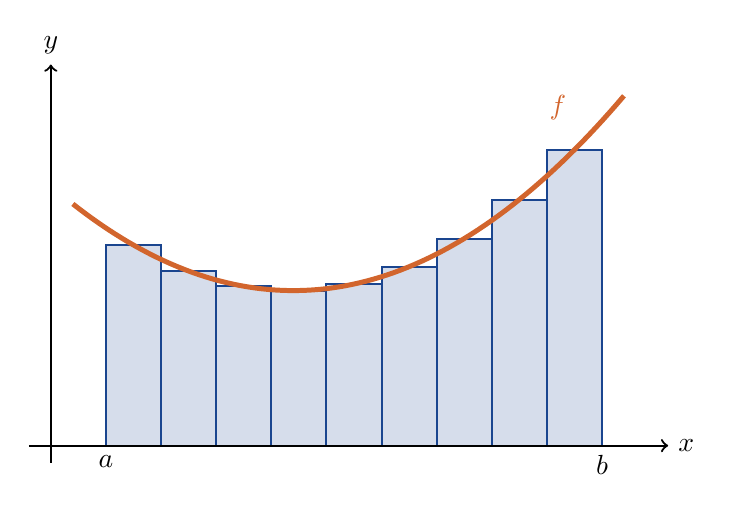
\begin{tikzpicture}[x=1.4cm,y=1.1cm]
  \foreach \x in {0.5,1,...,4.5}
    \draw[fill=tb,fill opacity=0.18,draw=tb,line width=0.7pt]
      (\x,0) rectangle +(0.5,{0.25*(\x+0.25)*(\x+0.25)-1.1*(\x+0.25)+3});
  \draw[->,line width=0.8pt] (-0.2,0) -- (5.6,0) node[right] {$x$};
  \draw[->,line width=0.8pt] (0,-0.2) -- (0,4.4) node[above] {$y$};
  \draw[to,line width=1.8pt,domain=0.2:5.2,samples=80] plot (\x,{0.25*\x*\x-1.1*\x+3});
  \node[below] at (0.5,0) {$a$}; \node[below] at (5,0) {$b$};
  \node[to] at (4.6,3.9) {$f$};
\end{tikzpicture}
